\chapter{晶体生长热力学}
\authors{唐棣生\quad 李沈军}
晶体生长是一门古老的“艺术”,但最近几十年来,由于热力学、统计物理以及其他学科在晶体生长中的应用,对解决晶体生长问题发挥了很大的作用,使晶体生长获得了牢固的科学基础,逐步发展成为材料科学中的一个重要分支,对解决工业与科研所需的材料问题做出了重要的贡献。因此,要想了解和掌握晶体生长这门学科,首先就必须掌握热力学的基本知识。

晶体生长是一个动态过程,不可能在平衡状态下进行,而热力学所处理的问题一般都是属于平衡状态问题。这两者结合到一起似乎有些矛盾。不过,在研究任何过程的动力学问题之前,对其中所包含的平衡问题有所了解,则可以预测过程中所遇到的问题(例如偏离平衡状态的程度),以及说明或提出解决问题的线索,因而在考虑实际晶体生长状况时,必须确定问题的实质究竟是与达到的平衡状态有关,还是与各种过程进行的速率有关。如果晶体生长的速率或晶体的形态取决于某一过程进行的速率(例如,在表面上的成核速率),那么就必须用适当的速率理论来分析,这时热力学就没有什么价值了。但如果过程进行程度非常接近于平衡态(准平衡态,这在高温时常常是如此),那么热力学对于预测生长量,以及成分随温度、压力和实验中其他变数而改变的情况,就有很大的价值。

实际上,可以认为晶体生长是控制物质在一定的热力学条件下进行的相变过程。

\section{相平衡及相变}
所谓相,是指体系中均匀一致的部分,它与别的部分有明显的分界线。例如,在大气压力下,冰与水混合共存时,冰本身是均匀一致的,它与水总有一定的分界面。不管是一大块冰,还是许多小冰块,冰所表现的物理状态和和化学状态总是一样的。所以在这个体系中,冰是一个相,水是另一个相。有时在同一种物质的固体状态(例如冰)下,由于温度或/和压强的不同,也可能有不同的结构(对称性)存在。这时候同时一种物质在固态下的不同结构,我们认为也是属于不同的相。但是在气体状态时,无论是由单一种气体或是几种不同气体组成,都是单一个相。

两相处于平衡状态时,其宏观性质有什么关系呢?我们可以根据热力学中的平衡判据来求出。
\subsection{热平衡}
设将$A$和$B$两个相封闭在一个与环境隔绝(与环境无热量和物质的交换)的体系内,$A$与$B$两相之间只有热量交换,即$A,B$两相间的隔板完全固定,只能导热。如图1.1所示,设此时从$A$有微量的热传到$B$内,则$A,B$两相的内能变化为
\begin{equation}
\begin{aligned}
\mathrm{d}U_A-T_AdS_A-P_AdV_A, \\
\mathrm{d}U_B-T_BdS_B-P_AdV_B
\end{aligned}
\end{equation}
由于隔板固定,故$A,B$两相的体积也固定,故$dV_A=dV_B=0$。
\begin{figure}[h]
 \centering
 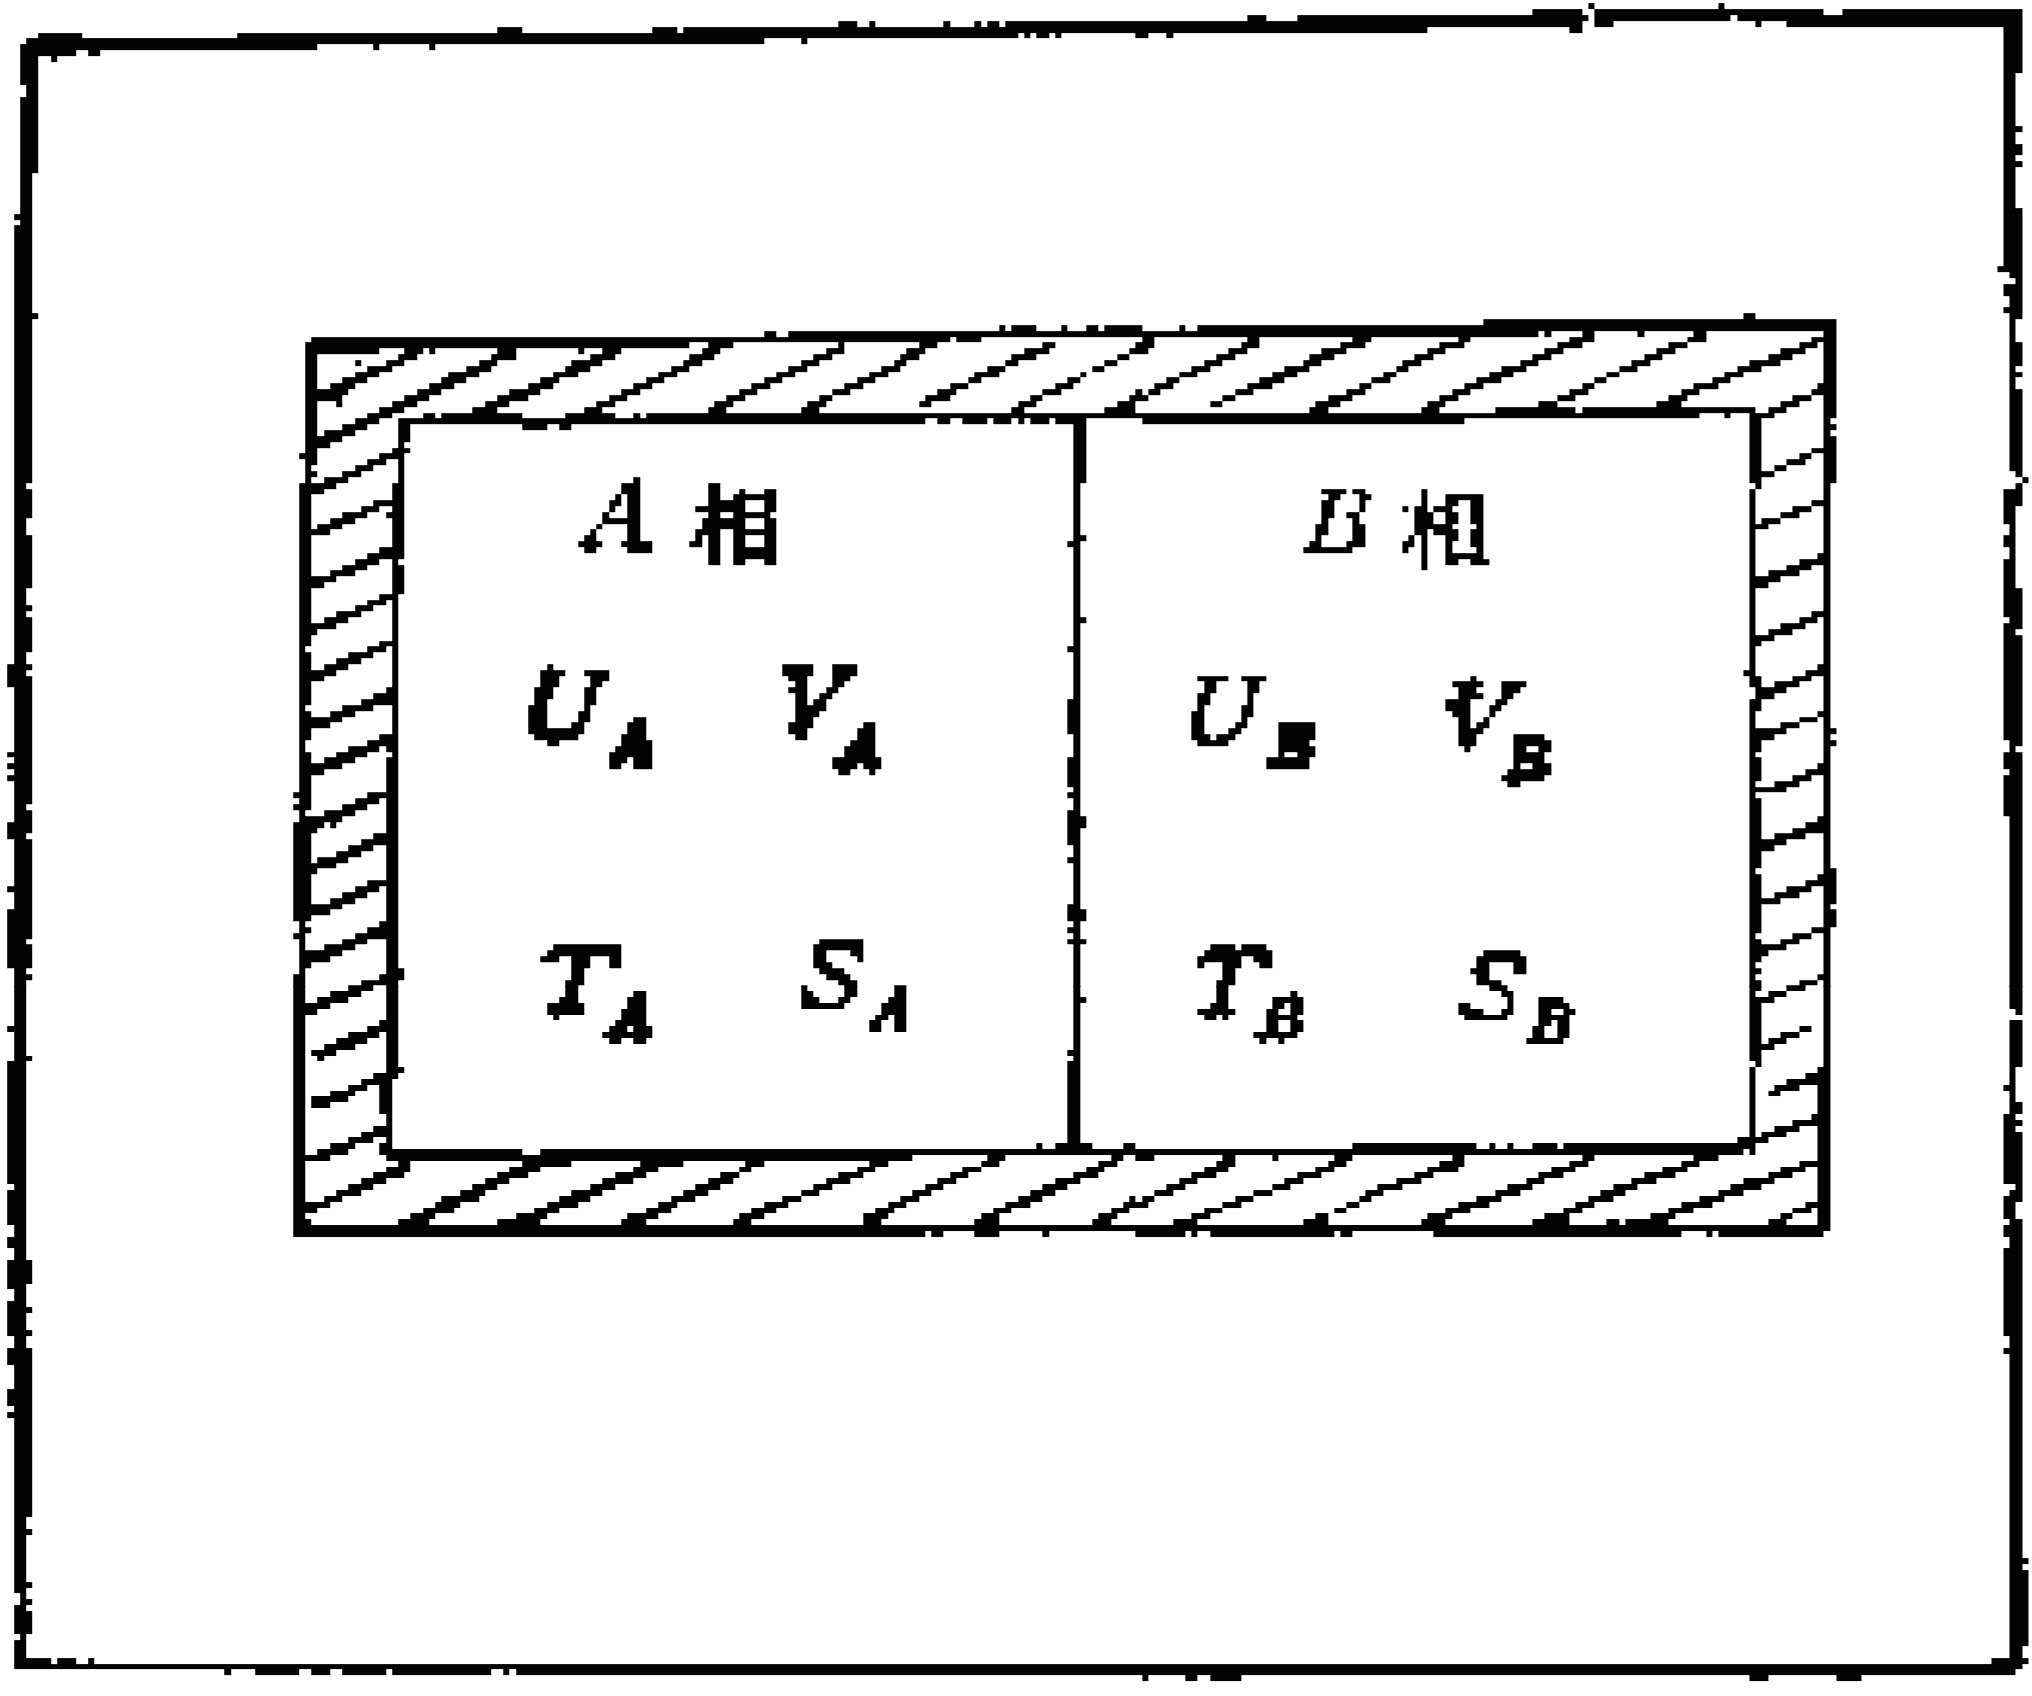
\includegraphics[width=0.4\textwidth]{fig/cp01/img1.1.jpg}
 \caption{推导两相间热平衡所用示意图。}
\end{figure}
这说明此时体系内能的变化只表现为热的改变,即
$$\delta Q=-dU_A=dU_B.$$
这里假定由$A$传至$B$时,对$B$相来说,$\delta Q$为正,反方向为负。于是式(1.1)可写为
\begin{equation}
-\delta Q/T_A=dS_A,\ \ \delta Q/T_B=dS_B.
\end{equation}
两式相加,得
$$\frac{\delta Q(T_A-T_B)}{T_AT_B}=dS_A+dS_B=d(S_A+S_B)\geq 0$$
不平衡时,$d(S_A+S_B)>0$,即$T_A>T_B$,热量由高温传至低温。当体系处于平衡态时,熵应为最大,也即$d(S_A+S_B)=0$,于是得出$\delta Q(T_A-T_B)=0$,但$\delta Q\neq 0$,故有
\begin{equation}T_A=T_B\end{equation}
这就是说,两相在互相接触的情况下达到平衡时,温度应该相等。 %热平衡
\subsection{力学平衡}
若两相都为流体时,我们将它们放置在一个恒温恒容箱内。根据自由能判据,得出平衡状态时应有
$$dF=dF_A+dF_B=0.$$
设两相之间无物质交换,但可改变体积,则
\begin{equation}
\begin{aligned}
dF_A&=-S_AdT_A-P_AdV_A, \\
dF_B&=-S_BdT_B-P_BdV_B.
\end{aligned}
\end{equation}
由于恒温,故$dT_A=dT_B=0$;由于总体积不变(恒容),故$dV=dV_A+dV_B=0$,得$dV_A=-dV_B$,于是$dF=dF_A+dF_B=\left(P_A-P_B\right)dV_A=0$。但$dV_A\neq 0$,故
\begin{equation}
P_A=P_B.
\end{equation}
这就是说,当两相在恒温,且总体积不变(恒容)的情况下处于平衡状态时,两相的压强应相等,这里假设两相间的接触面是平面,如果接触面是弯曲界面(如图1.2所示),且$A$相是球体时,则应加入表面能项,即$dF_A$中除了$P_AdV_A$外,还有$\sigma d\alpha_A$项,$\sigma$表示比表面能,$\alpha_A$表示$A$相的表面积。

(图1.2)

\noindent 于是
\begin{align*}
dF_A&=-S_AdT_A-P_AdV_A+\sigma d\alpha_A,\\
dF_B&=-S_BdT_B-P_BdV_B,
\end{align*}
将$dV_B=-dV_A$代入,则两式相减后,得
$$-(P_A-P_B)dV_A+\sigma d\alpha_A=0$$
故
$$P_A-P_B=\frac{\sigma d\alpha_A}{dV_A}.$$
由于球体的$\dfrac{d\alpha_A}{dV_A}=\dfrac{2}{R}$,代入后,得
\begin{equation}
P_A-P_B=\frac{2\sigma}{R}
\end{equation}
当$R\rightarrow\infty$,即曲面变为平面时,式(1.6)即变为式(1.5)。 %力学平衡
\subsection{传质平衡}
 %传质平衡
\subsection{相律}
当我们研究一个体系时,一般说来,它是由不同的元素或化合物所组成的。这些组成的元素或化合物形成不同的相(可能是一种或多种)。在不同的条件(压力、温度、浓度)下,体系达到平衡时所出现的相的数目也会有所不同。我们感兴趣的是,这些变量之间究竟存在什么样的关系。掌握了这个关系,我们就能了解、掌握和控制体系向着所需要的方向变化和发展。相律就是表示这种关系的一个方程式。它表示一个多相平衡体系的自由度与相数、组元数及影响平衡的外界条件数目之间的关系。也就是说,必须知道要有多少的条件才能决定体系的状态,实际上这就是一个众所周知的代数定理(即必须有$n$个方程式才能确定$n$个变数的数值)在物理化学中的具体应用。

关于相的概念在前面我们已经讲过,现介绍组元数的概念。任何一个体系总包含一些不同的元素及化合物,我们把这些元素和化合物称作组分。凡在体系内可以独立变化,而且决定着各相成分的组分就称为这个体系的组元。在没有组分间关系的限制条件时,体系的组元数就等于它的组分数。如果体系内有化学反应或存在其他的组分间关系的限制条件(如某几个组分间浓度之比固定等)时,那么它的组元数就不等于它的组分数,而是等于组分数减去组分间关系的限制条件数。例如,$\rm LiIO_3$水溶液,组分数为$2$(即$\rm LiIO_3$和水),组元数亦为$2$。而$\rm NaCl$和$\rm KNO_3$的水溶液,存在着一个化学反应
$$\rm NaCl + KNO_3 \rightleftharpoons NaNO_3+KCl,$$
这个体系共含有5个组分($\rm NaCl,KNO_3,NaNO_3,KCl,H_2O$)。但由于其中有一个化学反应,同时$\rm NaNO_3$和$\rm KCl$是反应的产物,且其浓度比必为$1:1$,所以这个体系的组元数为3(可以认为是$\rm H_2O,NaCl,KNO_3$或$\rm H_2O,NaNO_3,KCl$)。水、冰、水蒸气组成的体系,则是一个组分($\rm H_2O$),也是一个组元。我们把由一个组元组成的体系称为单元系,两个组元组成的体系称为二元系。其他的依此类推。

关于自由度数的概念,它是指一个平衡体系的可变因素(例如每一相的温度、压力、成分等)的数目。这些因素在一定范围内可以任意改变,而不使任何原有的相消失,也不使任何新相产生。例如,单组元的水体系,在一定范围内压力与温度可以任意改变,而不产生水蒸气或冰,这时我们称它有两个自由度(体系内只有水这一个相)。又如水和水蒸气平衡共存(两相共存)的单组元体系内,由于温度和压力存在一定的关系($\mu_\text{水}(T,P)=\mu_\text{汽}(T,P)$),所以两者之中只有一个可以在一定范围内变化,否则就将导致某一相的消失。这样,这个体系的自由度就只有一个。而水、冰、水蒸气三相平衡的单元系中,这3个相只有在固定的温度和压力下才能平衡共存,这个体系没有任何可变的因素,我们称它是自由度为零的不变体系。

下面来推导相律的表达式。在一个不存在化学反应的体系中,设有$c$个组分,分布在$\phi$个相中。要确定一个相的状态必须知道该相的温度、压力以及$(c-1)$个浓度的值(浓度采用摩尔百分数表示,$c$个组分浓度之和为$100\%$)。因此,要知道整个体系的状态,就必须知道$\phi$个相中的温度、压力及组分浓度,这样必须了解下列各相的数值:
$$
\left.
\begin{aligned}
&P^a,& &T^a,& &(c-1)^a&\text{ 个浓度},\\
&P^b,& &T^b,& &(c-1)^b&\text{ 个浓度},\\
&\hspace{0.5em}\vdots&&\hspace{0.5em}\vdots&&\hspace{1.5em}\vdots&\\
&P^\phi,& &T^\phi,& &(c-1)^\phi&\text{ 个浓度},
\end{aligned}
\right\}
\begin{aligned}
&\text{式中}a,b,\cdots,\phi\text{等}\\
&\text{表示}a\text{相},b\text{相},\cdots\phi\text{相等(不是幂指数)。}
\end{aligned}
$$
但在平衡时,$P^a=P^b=\cdots=P^\phi=P,\ T^a=T^b=\cdots=T^\phi=T$,所以只需要知道$\{\phi(c-1)+2\}$个变数的数值就够了。

另外,根据相平衡的条件,每个组份在各相中的化学势相等,有
$$\begin{matrix}
\mu_1^a&=&\mu_1^b&=&\cdots&=&\mu_1^\phi,&\text{共}&(\phi-1)&\text{个等式},\\
\mu_2^a&=&\mu_2^b&=&\cdots&=&\mu_2^\phi,&\text{共}&(\phi-1)&\text{个等式},\\
\vdots&&\vdots&&\vdots&&\vdots&&\vdots&\\
\mu_c^a&=&\mu_c^b&=&\cdots&=&\mu_c^\phi,&\text{共}&(\phi-1)&\text{个等式}.
\end{matrix}$$
上列各式中的下标$1,2,\cdots,c$表示组元数,所以共有$c(\phi-1)$个方程式。确定由$\phi$个相组成的体系的状态所需要的变数数目与已有的方程式数目之差为
$$\phi(c-1)+2-c(\phi-1)=c+2-\phi.$$
这个结果的物理意义是,要想确定$\phi$个相的状态时,需要知道$(c+2-\phi)$个状态变数的数值。例如,上面提到的水、水蒸气这个两相共存的体系,$\phi=2$而$c=1$,故$c+2-\phi=1$,也就是说,影响相的存在的变数中,例如压力、温度、组分浓度(因是单元系,故组分不能变),只有压力和温度这两者之一才是可变的,即自由度为1。以$f$代表自由度数,上面的结果可以写为
\begin{equation}
f=c+2-\phi
\end{equation}

应用相律时要注意以下几点:
\begin{enumerate}[(1)] \itemsep -0.5ex
\item 这个式子推导时要求体系处于平衡状态,因此只适用于平衡状态的体系。
\item 这个式子的数目字$2$,表示整个体系的温度、压力均匀一致,所以是两个变数。若遇到不符合此条件的体系时(如渗透体系),即需补充变数。
\item 只以$T,P$为外界变数,就意味着忽略电磁力、表面力、重力等效应。虽然实际情况中有很多是与此相符合的,但不可忘记也有与事实不符的可能性。
\item 自由度只取零以上的正值,不能取负值。如出现$f$取负值时,说明体系可能处于非平衡状态。
\end{enumerate}
\newpage %相律
\subsection{相变}
 %相变

